% Copyright (c) 2012 by Michał Nazarewicz <mina86@mina86.com>
% Distributed under the terms of the Creative Commons
% Attribution-ShareAlike 3.0 Unported (CC BY-SA 3.0) license.

\subsection{Alokator stron}

\begin{frame}
  \frametitle{Algorytm bliźniaków}
  \begin{columns}[c]

    \column{0.6\textwidth}
    \begin{itemize}
    \item Alokator stron implementuje algorytm bliźniaków.
    \item Żądania w~kategoriach rzędu strony.
    \item Rząd może być 0--10\textcolor{gray}{$^\dagger$}.
    \item Zbyt duże strony są dzielone na połowy (tzw.\ bliźniaków).
    \item Podczas zwalniania, strona jest łączona z~bliźniakami.
    \end{itemize}

    \column{0.4\textwidth}
    \begin{center}
    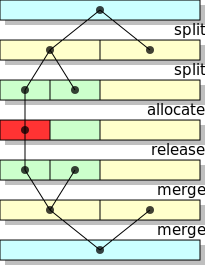
\includegraphics[width=0.9\textwidth]{build/alloc-free-cycle.eps}
    \end{center}
  \end{columns}
\end{frame}

\begin{frame}
  \frametitle{Strony i~bloki stron}
  \begin{center}
  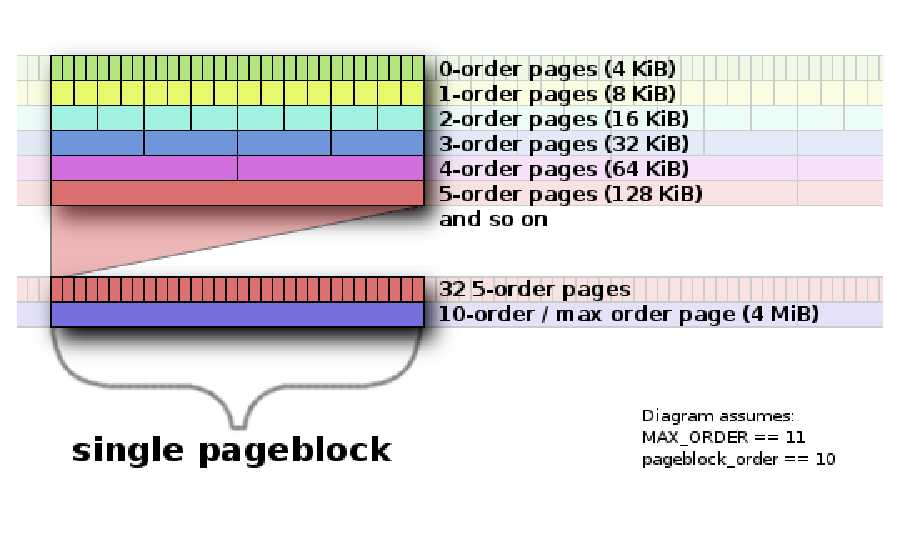
\includegraphics[width=0.9\textwidth]{build/pages.eps}
  \end{center}
\end{frame}

\begin{frame}[fragile]
  \frametitle{Typy migracji stron}

  \begin{itemize}
  \item Przy alokacji, użytkownik określa typ migracji żądanej strony:
    \begin{itemize}
    \item \textit{unmovable}, \textit{reclaimable} lub \textit{movable}.
    \end{itemize}
  \item Dla potrzeb CMA:
    \begin{itemize}
    \item \textit{unmovable} i \textit{reclaimable} $\rightarrow$ strony
      \textsl{nieruchome},
    \item \textit{movable} $\rightarrow$ strony \textsl{ruchome}.
    \end{itemize}
  \end{itemize}
\end{frame}

\begin{frame}[fragile]
  \frametitle{Typy migracji bloków stron}

  \begin{itemize}
  \item Każdy blok stron ma przypisany typ migracji.
  \item Przy alokacji strony są brane z~odpowiedniego bloku.
    \begin{itemize}
    \item Chyba, że takowych nie ma.
    \end{itemize}
  \item Ułatwia to trzymanie stron tego samego typu razem.
  \item Typ bloku może się zmieniać.
  \end{itemize}
\end{frame}

\begin{frame}[fragile]
  \frametitle{Migracja}

  \begin{itemize}
  \item Strony ruchome, mogą być migrowane.
  \item Migracja polega na:
    \begin{itemize}
    \item skopiowaniu zawartości strony gdzie indziej i
    \item uaktualnieniu odwołań do starej strony.
    \end{itemize}
  \item Przykładami stron ruchomych są:
    \begin{itemize}
    \item anonimowe strony procesów i
    \item bufory dyskowe.
    \end{itemize}
  \end{itemize}
\end{frame}
